
\documentclass{article}

\usepackage[french]{babel}
\usepackage[utf8]{inputenc}
\usepackage{graphicx}
%%%%%%%%%%%%%%%% Lengths %%%%%%%%%%%%%%%%
\setlength{\textwidth}{15.5cm}
\setlength{\evensidemargin}{0.5cm}
\setlength{\oddsidemargin}{0.5cm}

%%%%%%%%%%%%%%%% Variables %%%%%%%%%%%%%%%%
\def\projet{1}
\def\titre{Méthodes de calcul numérique }
\def\groupe{4}
\def\equipe{2}
\def\responsible{Kamgang Nintcheu David}
\def\secretary{Langlais Hugo}
\def\others{Roger Gaetan, Medina Enzo}


\begin{document}

%\maketitle

%%%%%%%%%%%%%%%% Header %%%%%%%%%%%%%%%%
\noindent\begin{minipage}{0.98\textwidth}
  \vskip 0mm
  \noindent
  { \begin{tabular}{p{7.5cm}}
      {\bfseries \sffamily
        Projet \projet} \\ 
      {\itshape \titre}
    \end{tabular}}
  \hfill 
  \fbox{\begin{tabular}{l}
      {~\hfill \bfseries \sffamily Groupe \groupe\ - Equipe \equipe
        \hfill~} \\[2mm] 
      Responsable : \responsible \\
      Secrétaire : \secretary \\
      Codeurs : \others
    \end{tabular}}
  \vskip 4mm ~

  ~~~\parbox{0.95\textwidth}{\small \textit{Résumé: } \sffamily 
  Ce
  projet consiste à étudier les calculs numériques sur machine. 
  La première partie se focalise sur l'erreur relative engendré par les calculs machines. 
  La seconde en revanche, étudie ...
\\ 
\\ }
  \vskip 1mm ~
\end{minipage}

%%%%%%%%%%%%%%%% Main part %%%%%%%%%%%%%%%%

\section*{Partie I - Représentation des nombres en machine}

\subsection*{Représentation décimale réduite}
Dans un premier temps, on crée la fonction rp(x, p) qui nous permet de récupérer la représentation décimale réduite d'un nombre en fonction d'une précision donnée. \\
Pour cela, nous récupérons d'abord la notation scientifique du nombre x. Puis nous sélectionnons seulement les p premières décimales de ce nombre et enfin nous multiplions le résultat obtenu par la puissance de dix perméttant un résultat du même ordre de grandeur que le x passé en paramètre.
\subsection*{Opérations usuelles en représentation décimale réduite}

Pour simuler les opérations usuelles (addition ou multiplication) en représentation décimale réduite, on crée une fonction qui prends en argument les deux nombres et la précision demandé (On part du principe que la précision est commune aux deux nombres). \\
On commence par récupérer la représentation décimale réduite des deux nombres via la fonction précédente. Ensuite, on calcule la somme (resp. multiplication) et on en calcule la représentation décimale réduite. On est obligé de réutiliser la fonction car la somme (resp.multiplication) de deux nombres ne donne pas nécessairement un nombre avec la bonne précision. \\
\newline
Par exemple : \\
Une précision de 3 sur les nombres 8.547 et 3.589 nous donne 8.54 et 3.59. En les sommant, on obtiens 12.13 qui à une précision de 4. On est donc bien obligé d'appeler une seconde fois la fonction rp() pour une obtenir une précision de 3.

\subsection*{Erreur relative}

On calcule l'erreur relative de la somme et de la multiplication donné par les formules : \\
\\
Erreur relative sur la somme:
\begin{equation}
\delta_{s}(x,y) = \frac{ \left |  (x+y)_{reel}\ - \ (x+y)_{machine} \right | }{\left |  (x+y)_{reel} \right | }
\end{equation}
\\
Erreur relative sur le produit:
\begin{equation}
\delta_{p}(x,y) = \frac{ \left |  (x*y)_{reel}\ - \ (x*y)_{machine} \right | }{\left |  (x*y)_{reel} \right | }
\end{equation}


Ici, on considère le résultat "réel" comme étant celui calculé par python. Le résultat machine correspond à notre calcul précédent. On arrive alors à obtenir une erreur relative qui nous permet d'examiner la précision de notre calcul. 
Sans surprise, plus la précision est forte, plus l'erreur relative est faible.

\subsection*{Graphes d'erreur relative}

On pose une précision égale à 3 pour n'avoir ni une précision trop forte (impliquant une erreur relative trop faible) ni une précision trop faible (impliquant une erreur relative trop forte).

Ci-dessous les graphes des erreurs relatives ${x = 1}$, soit une précision supérieure aux décimales du nombre, et ${x = 5.7555}$ soit une précision inférieure aux décimales du nombre. On remarque que l'erreur est maximal quand la somme à calculer est nul. De plus cette erreur est bien plus garnde dans le cas où ${x=5.7555}$ que dans le cas où ${x=1}$ cela peut s'expliquer par le fait que dans ce deuxième cas x possède plus de décimales que la précision choisi ainsi le nombre étant tronqué l'erreur relative en sera donc augmentée. 


\begin{figure}[ht]
    \centering
    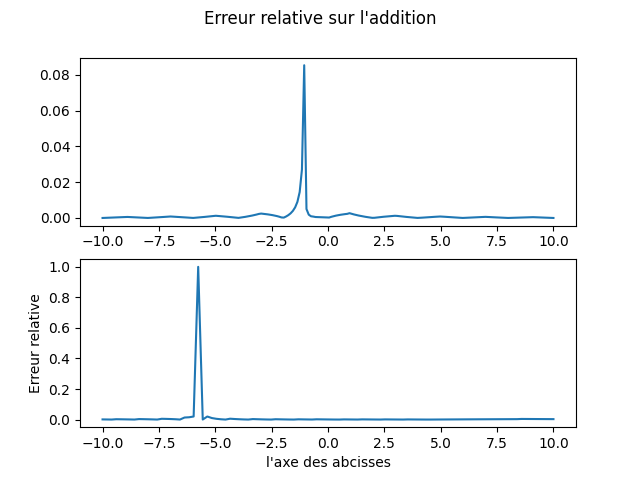
\includegraphics[scale=0.6]{erreur_add.png}
    \caption{Erreur relative sur la somme}
    \label{fig:erreur_add}
\end{figure}

Nous avons conservé les mêmes valeurs de x pour l'erreur relative sur le produit. On peut remarquer que les résultats sont bien moins prévisibles et que surtout l'erreur relative atteinte est beaucoup plus faible. 

\begin{figure}[ht]
    \centering
    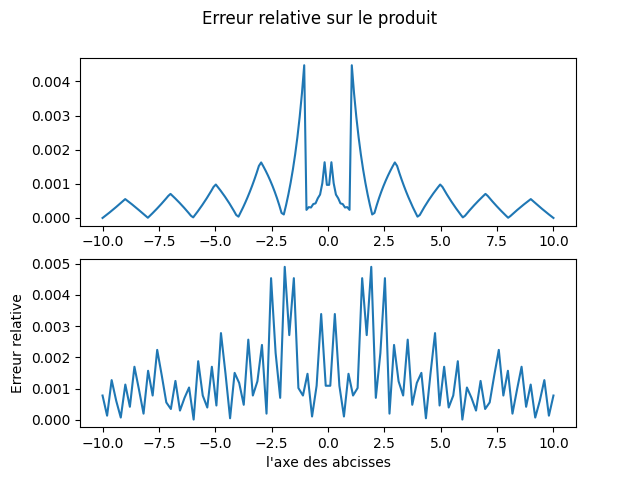
\includegraphics[scale=0.6]{erreur_prod.png}
    \caption{Erreur relative sur le produit}
    \label{fig:erreur_prod}
\end{figure}


\subsection*{Logarithme}

On commence par simplifier l'équation de $log(2)$.

\begin{equation}
log(2) = \sum_{n=1}^{\infty}\frac{(-1)^{n+1}}{n}
\end{equation}

\begin{equation}
\frac{1}{n}-\frac{1}{n+1}=\frac{1}{n(n+1)} \rightarrow log(2) = \sum_{k=1}^{\infty}\frac{1}{2k(2k-1)}
\end{equation}

\begin{equation}
log(2) \simeq \sum_{k=1}^{N}\frac{1}{2k(2k-1)}
\end{equation}

\begin{equation}
\epsilon
=
\left |  
log(2)-
\sum_{k=1}^{N}\frac{1}{2k(2k-1)}
\right |
=
\left |  
\sum_{n=1}^{\infty}\frac{(-1)^{n+1}}{n}-
\sum_{n=1}^{2N}\frac{(-1)^{n+1}}{n}
\right |
=
\left |  
\sum_{n=2N+1}^{\infty}\frac{(-1)^{n+1}}{n}
\right |
\end{equation}

\begin{equation}
    \epsilon \leq \frac{1}{2N+1} 
\end{equation}

Pour obtenir une précision sur p décimales, on a besoin d'aller à un N égale à ${10^{p}}$. 


Dès lors que l'on arrive à calculer un logarithme approché (en fonction de la précision), on peut en déduire l'erreur relative en fonction de la précision. On affiche sur un graphe l'erreur relative jusqu'à la précision 6 (On ne voit plus de différence avec une précision 7 ou au dessus, l'erreur relative étant inférieur à ${1.10^{-6}}$.


\begin{figure}[!ht]
    \centering
    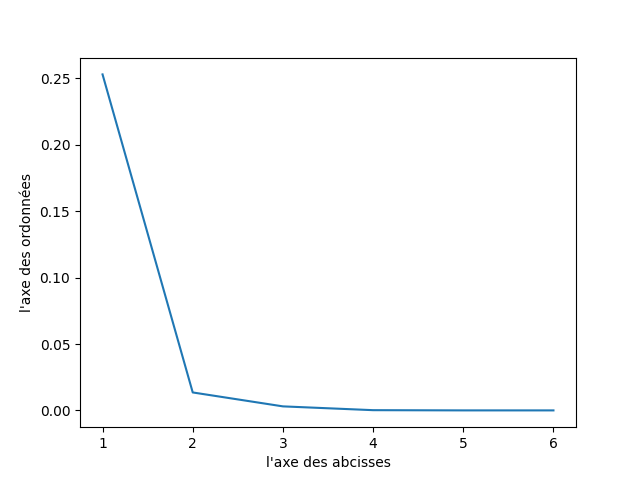
\includegraphics[scale=0.5]{erreur_relative.png}
    \caption{Erreur relative du log en fonction de la précision}
    \label{fig:log_prec}
\end{figure}

\begin{figure}[!ht]
    \centering
    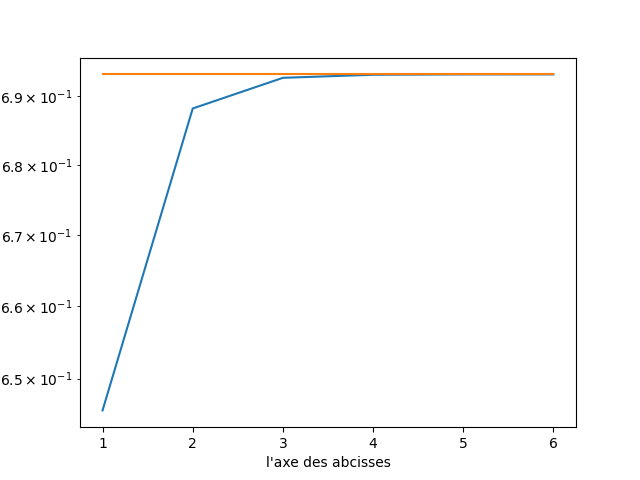
\includegraphics[scale=0.5]{graphes_log.png}
    \caption{Les deux log calculés, valeur réelle et valeur approchée en fonction de la précision}
    \label{fig:compare_log}
\end{figure}




\section*{Partie II}

Algorithmes CORDIC :


1) citer le chapitre ?

2) Quelle est la représentation des nombres utilisés sur une calculatrice ? Quels avantages et inconvénients pouvez-vous voir à ce genre de représentation ?

Dans une calculatrice, les nombres sont représentés en Binaire Code Decimal. Son principe : Les nombre sont représentas par des nombres décimaux et chaque chiffre est codé sur 4 bits.\\
Exemple :\\
12 en binaire est : 1100\\
1 en BCD est : 0001\\
2 en BCD est : 0010\\
donc 12 en BCD est : 0001 0010\\

Avanges :\\
- Multiplication et division par 10n plus rapide : shift left ou droit de 4*n bits.\\
- Toutes les fonctions 'standard' peuvent se ramener aux quatre fonctions suivantes :  ln, exp, tan, arcta n\\
- Calculs plus rapides grâce aux algorithmes de CORDIC\\
- Précision de plus de 12 chiffres avec seulement une quinzaine de valeurs précalculées.\\

Inconvénients :\\
- Multiplication et division par 2n plus lente que l'écriture binaire conventiennele : le shift de 1 bit ne multiplie ou divise plus.\\
- Pour un même nombre, prends plus de place en mémoire : besoin de nombre de chiffres * 4 bits contre log2(nombre) +1\\
- Pour utiliser les algorithmes de CORDIC, on a besoin de certains valeurs précalculées.\\

3) Dans cette page, quatre algorithmes sont décrits pour calculer les fonctions trigonométriques et exponentielles. Quelle est la technique générale utilisée pour réaliser ces algorithmes ? En particulier, en quoi cette technique vous semble t’elle efficace lorsqu’elle est ramenée à une calculatrice ?\\

Technique générale utilisée pour réaliser ces algorithmes :\\
- On décompose le nombre en produit partiel des valeurs précalculé (x pour ln, exp(x) pour exp). Et respectivement en somme partiel (atan(x), tan(x))) des valeurs précalculés.\\
-On se sert de ces produits (resp sommes) pour exploiter les developements  limités à l'ordre 1 des fonctions considérées pour se ramener à un résultat lénéaire facilement calculable par la calculatrice en valeur de retour. \\ 
-Point d'éfficacité : \\
-Le fait que la technique reside en grande partie sur l'exploitation de valeurs précaculer (tableaux L et A), permet déconomiser un grand nombres d'opérations calculatoires.\\
-Les seuls opérations de multiplications utilisés sont faites avec des puissances de $10^{-1}$ qui deviennent vites très proches de 0, mais comme les nombres sont représentés en bases décimal, cela devient un avantage pour cette technique.
-L'algorithme converge rapidement car en 





\end{document}
